\scanpage{7}
\mspage{6}
\mspage{-3-}
\uline{Corollaire} (18.9.5) .- \uline{Sous les hypothèses de} (18.9.4), \uline{le foncteur}
\[
(18.9.5.1)\qquad Z\rightsquigarrow Z\otimes_A A'
\]
\uline{de la catégorie des préschémas étales sur} $X$, \uline{dans celle des préschémas étales sur} $X'$, \uline{est pleinement fidèle}.

Soient $Z_1,Z_2$ deux préschémas étales sur $X$, et\deleted{\unsure{X}} posons $Z_{\unsure{1|i}}'=Z_{\unsure{1|i}}\otimes_A A'$ $(\unsure{1|i}=1,2)$ ; \deleted{\illegible{2}} il s'agit de prouver que tout $X'$-morphisme $Z_1'\to Z_2'$ provient, par changement de base, d'un \inserted{$X$-}morphisme unique $Z_1\to Z_2$. Supposons d'abord que \deleted{$Z_1$ et} $Z_2$ soi\deleted{en}t \uline{séparé\deleted{s}} sur $X$ ; alors, comme $\operatorname{Hom}_X(Z_1,Z_2)$ s'identifie à \deleted{\illegible{1}} $\Gamma(Z_1\times_X Z_2/Z_1)$, et que $Z_1\times_X Z_2$ est étale et séparé sur $Z_1$, $\operatorname{Hom}_X(Z_1,Z_2)$ s'identifie fonctoriellement, en vertu de (17.9.3), à l'ensemble des parties ouvertes et fermées $U$ de $Z_1\times_X Z_2$ telles que la restriction à $U$ de la projection $p:Z_1\times_X Z_2\to Z_1$ soit un morphisme surjectif et radiciel. L'assertion résulte donc dans le cas considéré de (18.9.4) et de ce que $Z_1'\times_{X'}Z_2'= {}=(Z_1\times_X Z_2)\otimes_A A'$.
\margin{\figure{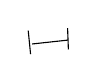
\begin{tikzpicture}[x=1cm,y=1cm]\draw (0,0)--(-.03,.3) (.02,.13)--(.48,.18) (.48,.06)--(.47,.33);\end{tikzpicture}}}

Passons au cas général ; il suffira de prouver que le graphe $\Gamma'$ d'un $X'$-morphisme $Z_1'\to Z_2'$, \inserted{qui est \uline{ouvert} (17.9.3) \inserted{dans $Z_1'\times_{X'}Z_2'$}} est de la forme $\Gamma\otimes_A A'$, où $\Gamma$ est \deleted{\illegible{1}} induit sur une partie \uline{ouverte} de $Z=Z_1\times_X Z_2$. En effet, la restriction à $\Gamma$ de la projection $p:Z\to Z_1$ est alors un \uline{isomorphisme}, car par changement de base \inserted{$A\to A'$} cette restriction devient l'isomorphisme restriction à $\Gamma'$ de la projection $p':Z'\to Z_1'$ (avec $Z'=Z\otimes_A A'$), et il suffit d'appliquer (2.7.1,(viii)) ; la conclusion résulte donc \inserted{alors} de la caractérisation des graphes de morphismes (\uline{I},5.3).
\margin{\figure{\begin{tikzpicture}[x=1cm,y=1cm]\draw (0,0) .. controls (.15,.18) and (.27,.2) .. (.4,.18) .. controls (.51,.16) and (.55,.25) .. (.52,.36);\end{tikzpicture}}}

Si $q:Z'\to Z$ est la projection canonique, pour prouver que $\Gamma'$ est de la forme \deleted{\illegible{1}} $q^{-1}(\Gamma)$, où $\Gamma$ est ouvert \inserted{dans $Z$}, il suffit, puisque $q$ est un morphisme \inserted{fidèlement} plat \inserted{et quasi-compact}, de prouver \deleted{\illegible{1}} qu'il existe un ensemble $U\subset Z$ tel que $\Gamma'=q^{-1}(\unsure{U})$ (2.3.12). Posons $Z''=Z'\times_Z Z'=Z\times_X X''$, où $X''=X'\times_X X'$, et soient $q_1:Z''\to Z'$, $q_2:Z''\to Z'$ les projections canoniques. Appli-
